% !TEX encoding = UTF-8 Unicode
\documentclass[
10pt,
aspectratio=169,
]{beamer}
\setbeamercovered{transparent=10}
\usetheme[
%  showheader,
%  red,
  purple,
%  gray,
%  graytitle,
  colorblocks,
%  noframetitlerule,
]{Verona}

\usepackage[T1]{fontenc}
\usepackage[utf8]{inputenc}
\usepackage{lipsum}
%%%%%%%%%%%%%%%%%%%%%%%%%%%%%%%
% Mac上使用如下命令声明隶书字体,windows也有相关方式,大家可自行修改
%\providecommand{\lishu}{\CJKfamily{zhli}}
%%%%%%%%%%%%%%%%%%%%%%%%%%%%%%%
\usepackage{tikz}
\usetikzlibrary{shapes,snakes}
\usetikzlibrary{fadings}
\usetikzlibrary{arrows.meta}
%
%\setbeamertemplate{sections/subsections in toc}[ball]
%\usepackage{xeCJK}
\usepackage{listings}
\usepackage{caption}
\usepackage{subcaption}
\usefonttheme{professionalfonts}
\def\mathfamilydefault{\rmdefault}
\usepackage{amsmath}
\usepackage{multirow}
\usepackage{booktabs}
\usepackage{bm}
\setbeamertemplate{section in toc}{\hspace*{1em}\inserttocsectionnumber.~\inserttocsection\par}
\setbeamertemplate{subsection in toc}{\hspace*{2em}\inserttocsectionnumber.\inserttocsubsectionnumber.~\inserttocsubsection\par}
\setbeamerfont{subsection in toc}{size=\small}
\AtBeginSection[]{%
	\begin{frame}%
		\frametitle{Outline}%
		\textbf{\tableofcontents[currentsection]} %
	\end{frame}%
}

\AtBeginSubsection[]{%
	\begin{frame}%
		\frametitle{Outline}%
		\textbf{\tableofcontents[currentsection, currentsubsection]} %
	\end{frame}%
}

%% listing for python snips
\usepackage{listings}
\definecolor{codegreen}{rgb}{0,0.6,0}
\definecolor{codegray}{rgb}{0.5,0.5,0.5}
\definecolor{codepurple}{rgb}{0.58,0,0.82}
\definecolor{backcolour}{rgb}{0.95,0.95,0.92}
\lstdefinestyle{mystyle}{
    backgroundcolor=\color{backcolour},   
    commentstyle=\color{codegreen},
    keywordstyle=\color{magenta},
    numberstyle=\tiny\color{codegray},
    stringstyle=\color{codepurple},
    basicstyle=\ttfamily\footnotesize,
    breakatwhitespace=false,         
    breaklines=true,                 
    captionpos=b,                    
    keepspaces=true,                 
    numbers=left,                    
    numbersep=5pt,                  
    showspaces=false,                
    showstringspaces=false,
    showtabs=false,                  
    tabsize=2
}
\lstset{style=mystyle}


\title{Introducci\'on a Python}
\subtitle{Comandos b\'asicos y gr\'aficas en Python}
\author[L.M.]{Luis Alejandro Morales, Ph.D.}
\mail{lmoralesm@unal.edu.co}
\institute[UNAL]{Facultad de Ingenier\'ia\\
Universidad Nacional de Colombia}
\date{\today}
\titlegraphic[width=3cm]{logo_01u}{}

%%%%%%%%%%%%%%%%%%%%%%%%%%%%%%%%
% ----------- 标题页 ------------
%%%%%%%%%%%%%%%%%%%%%%%%%%%%%%%%
% New commands
\newcommand{\gi}{\texttt{Git}}
\newcommand{\gih}{\texttt{GitHub}}
%\newcommand{\co}[1]{\alert{\textbf{\large \texttt{#1}}}}
\newcommand{\co}[1]{\alert{\textbf{\texttt{#1}}}}

\tikzset{
    *|/.style={
        to path={
            (perpendicular cs: horizontal line through={(\tikztostart)},
                                 vertical line through={(\tikztotarget)})
            % is the same as (\tikztostart -| \tikztotarget)
            % but just to be safe: http://tex.stackexchange.com/a/29781/16595
            -- (\tikztotarget) \tikztonodes
        }
    }
}
\begin{document}



\maketitle

%%% define code
\defverbatim[colored]\lstI{
	\begin{lstlisting}[language=C++,basicstyle=\ttfamily,keywordstyle=\color{red}]
	int main() {
	// Define variables at the beginning
	// of the block, as in C:
	CStash intStash, stringStash;
	int i;
	char* cp;
	ifstream in;
	string line;
	[...]
	\end{lstlisting}
}
%%%%%%%%%%%%%%%%%%%%%%%%%%%%%%%%
% ----------- FRAME ------------
%%%%%%%%%%%%%%%%%%%%%%%%%%%%%%%%

%---
\section{Generalidades}
\begin{frame}[c]{?`Que es Python?}
Python es un \alert{lenguaje de programación interpretado}, \alert{orientado a objetos}, de \alert{ alto nivel} y con \alert{semántica dinámica}. Sus estructuras de datos integradas de alto nivel, combinadas con escritura dinámica y enlace dinámico, lo hacen muy atractivo para el \alert{desarrollo rápido de aplicaciones}, así como para su uso como \alert{lenguaje de secuencias de comandos} o  para \alert{conectar componentes existentes}. La \alert{sintaxis simple y fácil} de aprender de Python enfatiza la legibilidad y, por lo tanto, reduce el costo de mantenimiento del programa. Python admite \alert{módulos y paquetes}, lo que fomenta la \alert{modularidad} del programa y la reutilización del código. El intérprete de Python y la extensa biblioteca estándar están disponibles en formato fuente o binario sin costo para todas las plataformas principales y se pueden distribuir \alert{gratuitamente}.
\end{frame}

\begin{frame}[c]{?`Como se ejecuta python en su computador?}
\begin{columns}
\column{0.5\textwidth}
\centering
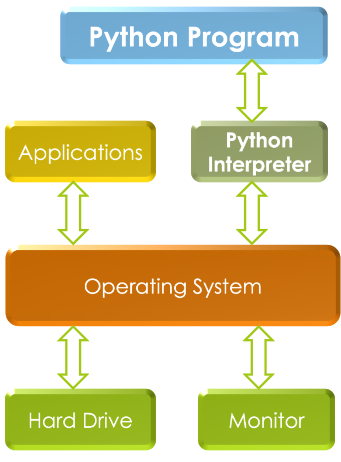
\includegraphics[width=0.75\textwidth]{fig1.png}
\column{0.6\textwidth}
\begin{itemize}
\item Python programs no se ejecutan directamente en el sistema opertativo (OS).
\item Otro programa llamado \alert{interprete} o \alert{m\'aquina virtual} toma el programa y lo pasa (ejecuci\'on) a lenguage de maquina (entendido por el OS).
\item Aqui se escribiran programas ejecutados por el interprete.
\end{itemize}
\end{columns}
\end{frame}

\begin{frame}[c]{?`Que tipo de lenguage es Python?}
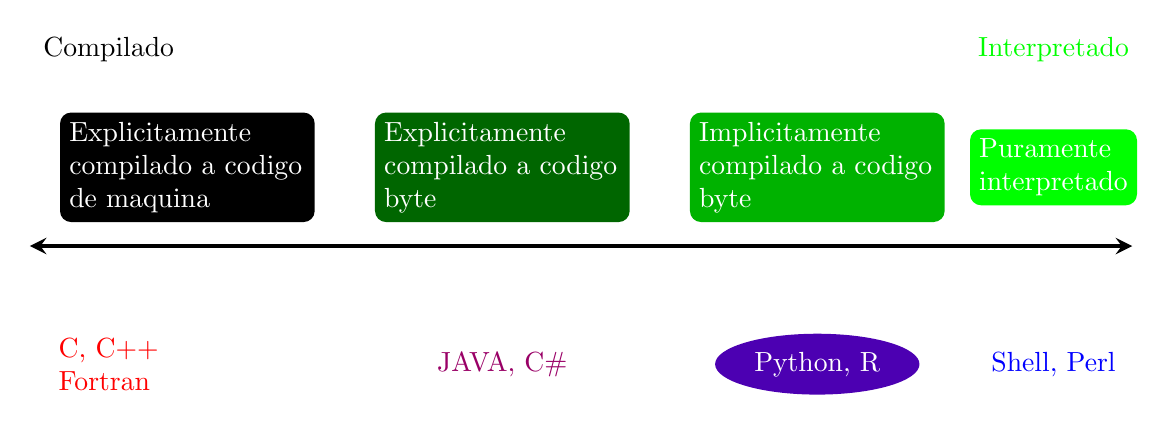
\begin{tikzpicture}
\node[text=black] at (-2,2.5) {Compilado};
\node[rounded corners,text width=3cm,fill=black,text=white] at (-1,1) {Explicitamente compilado a codigo de maquina};
\node[rounded corners,text width=3cm,fill=black!60!green,text=white] at (3,1) {Explicitamente compilado a codigo byte};
\node[rounded corners,text width=3cm,fill=black!30!green,text=white] at (7,1) {Implicitamente compilado a codigo byte};
\node[rounded corners,align=left,fill=green,text=white] at (10,1) {Puramente\\ interpretado};
\node[text=green] at (10,2.5) {Interpretado};
\draw [stealth-stealth, ultra thick](-3,0) -- (11,0);
\node[text=red,align=left] at (-2,-1.5) {C, C++\\ Fortran};
\node[text=red!60!blue] at (3,-1.5) {JAVA, C\#};
\node[ellipse,fill=red!30!blue, text=white] at (7,-1.5) {Python, R};
\node[text=blue] at (10,-1.5) {Shell, Perl};
\end{tikzpicture}
\end{frame}


\begin{frame}[c]{?`Para que sirve Python y sus ventajas?}
Untilidades de Python
\begin{itemize}
\item Science: Deterministic and statistical modelling
\item Instrumental control
\item Embedded systems
\item Web services
\item On-line games
\end{itemize}
Ventajas de Python
\begin{itemize}
\item Relativamente facil de aprender
\item Gran numero de librerias
\item Versatil e independiente de la plataforma
\item Comunidad con fuerte soporte
\end{itemize}
\end{frame}


\begin{frame}[c]{?`Como instalar Python?}
\begin{itemize}
\item Python tiene dos versiones:
\begin{itemize}
\item 2.x: Version m\'as antigua, carece de mantenimiento.
\item 3.x; Version reciente, con suporte actual. 
\end{itemize}
\item Minimo hardware requerido: $>$ 4GB de RAM, $>5$ GB de disco duro libre (para la instalaci\'on de librerias se requier m\'as espacio)
\end{itemize}
\begin{itemize}
\item Unix/Linux y Mac OS, Python viene instalado por defecto,:)

\item MS Windows
\begin{itemize}
\item Descargar el installador de Python en (\href{https://www.python.org/downloads/windows/}{https://www.python.org/downloads/windows/})
\item Ejecutar el installador \co{pytho3.x.x.exe}
\item Personalizar la instalaci\'on
\item Installar Python
\item Verificar la installaci\'on: Busque \co{cmd} y escriba \co{python --version}
\end{itemize}
\end{itemize}
\end{frame}

\begin{frame}[c]{?`Como usar Python?}
\begin{enumerate}
\item Ejecutar comandos y codigos directamente desde el interprete de Python

\begin{enumerate}
\item Abra la termninal (busque \co{cmd})
\item Ejecute \co{python3} o \co{python}. Producir\'a:
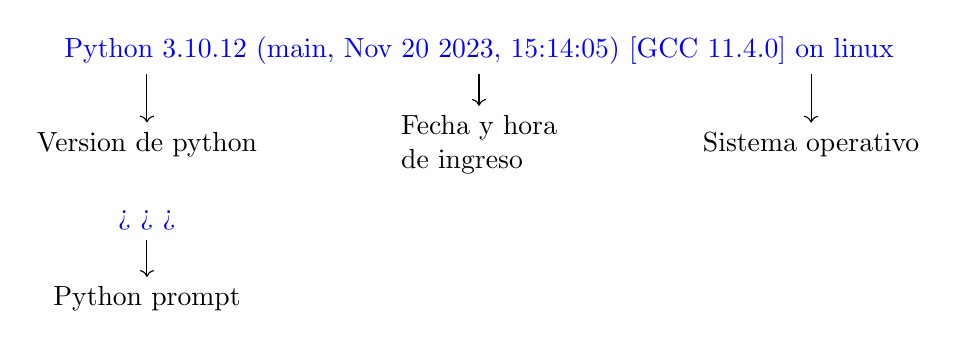
\begin{tikzpicture}[node distance=12em]
\node(G) [text=blue] {Python 3.10.12 (main, Nov 20 2023, 15:14:05) [GCC 11.4.0] on linux};
\node(H)  [align=left] [below=0.7cm] {Fecha y hora\\ de ingreso};
\node(H1) [left of=H]  {Version de python};
\node(H2) [right of=H] {Sistema operativo};
\draw[->,*|] (G.south) to     (H1.north);
\draw[->]    (G.south) --     (H.north);
\draw[->]    (G.south) to[*|] (H2.north);
\node(F) [text=blue,below of=H1, below=-3.5cm] {> > >};
\node(F1) [below of=F,below=-3.5cm] {Python prompt};
\draw[->,*|] (F.south) to     (F1.north);
\end{tikzpicture}
\end{enumerate}
\item Correr programas escritos en un archivo (e.g. \co{myprogram.py})
\begin{enumerate}
\item Abra la termninal (busque \co{cmd})
\item Para ejecutar el programa: \co{python3 myprogram.py} o \co{python myprogram.py}
\end{enumerate}
\item Salir de Python:
\begin{enumerate}
\item $> > >$ \co{exit()}
\item $> > >$ \co{quit()}
%\item \fbox{\begin{minipage} Ctrl \end{minipage}}
\item \fbox{Ctrl} + \fbox{D}
\end{enumerate}

\end{enumerate}

\end{frame}


\begin{frame}[c]{?`Como ejecutar un programa de Python?}
\begin{enumerate}
\item Abra un archivo nuevo en su editor de texto (e.g. \co{vi/vim}, \co{emacs}, \co{notepad})
\item Nombre su archivo como e.g. \co{myprogram.py}
\item Dentro de ese archivo escribir:
\begin{minipage}[t]{\linewidth}
\centering
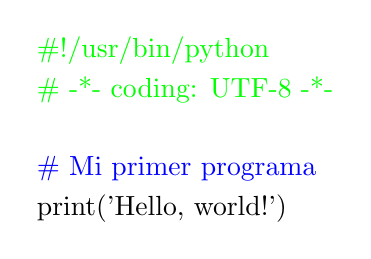
\begin{tikzpicture}
\node [anchor=west, text=green] at (0,1) {\#!/usr/bin/python};
\node [anchor=west, text=green] at (0,0.5) {\# -*- coding: UTF-8 -*-};
\node [anchor=west, text=blue] at (0,0) {};
\node [anchor=west, text=blue] at (0,-0.5) {\# Mi primer programa};
\node [anchor=west] at (0,-1.0) {print('Hello, world!')};
\end{tikzpicture}
\end{minipage}
\item En la consola de comandos, asegurese que usted esta en el directorio que contiene \co{myprogram.py}.
\item Ejecutar el programa como: \co{python3 myprogram.py} o \co{python myprogram.py}
\item Note que el \co{myprogram.py} puede leer parametros de entrada: \co{python3 myprogram.py} \co{para1} \co{para2} $\cdots$ \co{paran}

\end{enumerate}
\end{frame}

%---
\section{Comandos b\'asicos en Python}
\begin{frame}[c]{Primer comando en Python}
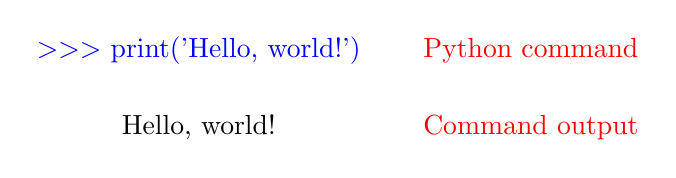
\begin{tikzpicture}[node distance=12em]
\node(G) [text=blue] {$> > >$ print('Hello, world!')};
\node(G1) [right of=G, text=red]  {Python command};
\node(H)  [align=left] [below=0.7cm] {Hello, world!};
\node(H1) [right of=H,text=red]  {Command output};
\end{tikzpicture}

\end{frame}

\begin{frame}[c]{Tipos de datos y operaciones en Python}
\begin{columns}
\column{0.7\textwidth}
\begin{itemize}
\item integers $\rightarrow$ $4$\ $15110$\ $-53$\ $0$
\item Floating point numbers $\rightarrow$ $4.0$ $0.80333333333$ $7.34e+014$
\item Strings  $\rightarrow$ "hello” "A" " " ”” 'there' '"' '15110'
\item Booleans $\rightarrow$ \texttt{True} \texttt{False}
\item Literal none $\rightarrow$ \texttt{None}
\end{itemize}
\column{0.3\textwidth}
\begin{itemize}
\item $+$ Addition 
\item $-$ Substraction 
\item $*$ Multiplication
\item $/$ Division
\item // Integer division
\item $**$ Exponentiation
\item \% Modulo (remainder)
\end{itemize}
\end{columns}
El interprete de python es como una calculadora:
\begin{minipage}[t]{\linewidth}
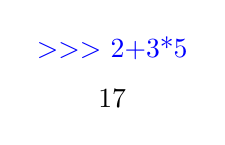
\begin{tikzpicture}
\node(G) [text=blue] {$> > >$ 2+3*5};
\node(H)  [align=right] [below=0.4cm] {17};
\end{tikzpicture}
\end{minipage}
Orden de evaluaci\'on de los operadores
\begin{minipage}[t]{\linewidth}
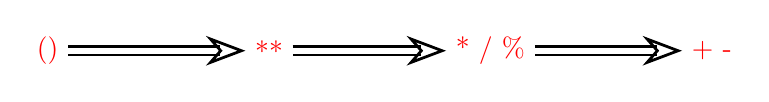
\begin{tikzpicture}[node distance=8em]
\node(A) [text=red] {()};
\node(B) [right of=A,text=red] {**};
\node(C) [right of=B,text=red] {* / \%};
\node(D) [right of=C,text=red] {+ -};
\draw[line width=1pt, double distance=2pt, -{Stealth[length=5mm, open]}]    (A.east) --     (B.west);
\draw[line width=1pt, double distance=2pt, -{Stealth[length=5mm, open]}] (B.east) --     (C.west);
\draw[line width=1pt, double distance=2pt, -{Stealth[length=5mm, open]}] (C.east) --     (D.west);
\end{tikzpicture}
\end{minipage}
\end{frame}


\begin{frame}[c]{Operaciones logicas}
\begin{columns}
\column{0.3\textwidth}
\begin{tabular}{c c}
Matem\'aticas & Python \\ \hline
$=$ & $==$ \\
$\neq$ & $!=$ \\
$<$ & $<$ \\
$>$ & $>$ \\
$\leq$ & $<=$ \\
$\geq$ & $>=$ 
\end{tabular}
\begin{minipage}[t]{\linewidth}
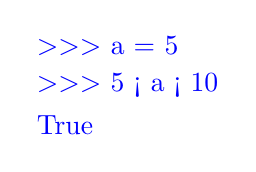
\begin{tikzpicture}
\node(A) [anchor=west, text=blue] at (0,0.5) {$> > >$ a = 5};
\node(B) [anchor=west, text=blue] at (0,0) {$> > >$ 5 < a < 10 };
\node(C) [anchor=west, text=blue] at (0,-0.5) {True};
\end{tikzpicture}
\end{minipage}

\column{0.7\textwidth}
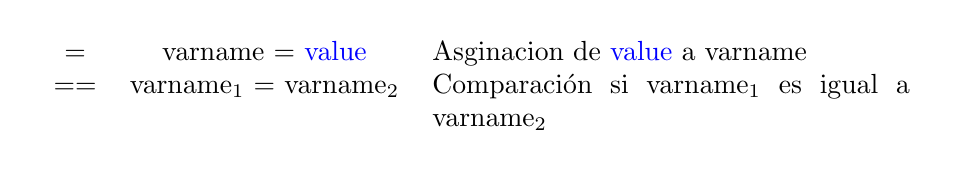
\begin{tikzpicture}
\node [align=center](A) at (4,0) {
\begin{tabular}{c c p{0.5\textwidth}}
$=$ & \alert{varname} = {\color{blue} value} & Asginacion de  {\color{blue} value} a \alert{varname}\\
$==$ & \alert{varname$_1$} = \alert{varname$_2$} & Comparaci\'on si \alert{varname$_1$} es igual a \alert{varname$_2$}
\end{tabular}};
\end{tikzpicture}
Operadores boleanos: \alert{and}, \alert{or} y \alert{not}
\begin{minipage}[t]{\linewidth}
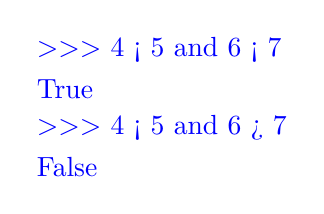
\begin{tikzpicture}
\node(A) [anchor=west, text=blue] at (0,0.5) {$> > >$ 4 < 5 and 6 < 7};
\node(B) [anchor=west, text=blue] at (0,0) {True};
\node(C) [anchor=west, text=blue] at (0,-0.5) {$> > >$ 4 < 5 and 6 > 7};
\node(D) [anchor=west, text=blue] at (0,-1) {False};
\end{tikzpicture}
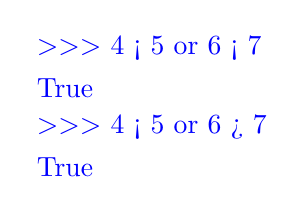
\begin{tikzpicture}
\node(A) [anchor=west, text=blue] at (3,0.5) {$> > >$ 4 < 5 or 6 < 7};
\node(B) [anchor=west, text=blue] at (3,0) {True};
\node(C) [anchor=west, text=blue] at (3,-0.5) {$> > >$ 4 < 5 or 6 > 7};
\node(D) [anchor=west, text=blue] at (3,-1) {True};
\end{tikzpicture}
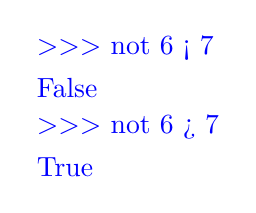
\begin{tikzpicture}
\node(A) [anchor=west, text=blue] at (0,-3.5) {$> > >$ not 6 < 7};
\node(B) [anchor=west, text=blue] at (0,-4) {False};
\node(C) [anchor=west, text=blue] at (0,-4.5) {$> > >$ not 6 > 7};
\node(D) [anchor=west, text=blue] at (0,-5) {True};
\end{tikzpicture}
\end{minipage}
\end{columns}

\end{frame}

\begin{frame}[c]{Expresiones y declaraciones}
\begin{itemize}
\item Python evalua una \alert{expresion} para obtener un resultado, e.g.:
\begin{minipage}[t]{\linewidth}
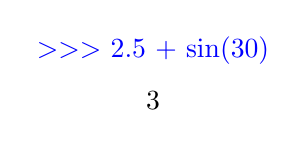
\begin{tikzpicture}
\node(G) [text=blue] {$> > >$ 2.5 + sin(30)};
\node(H)  [align=right] [below=0.4cm] {3};
\end{tikzpicture}
\end{minipage}

\item Python ejecuta una \alert{declaraci\'on} para realizar una acci\'on que tiene un efecto, e.g.:
\begin{minipage}[t]{\linewidth}
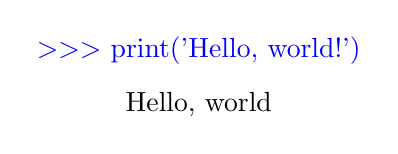
\begin{tikzpicture}
\node(G) [text=blue] {$> > >$ print('Hello, world!')};
\node(H)  [align=right] [below=0.4cm] {Hello, world};
\end{tikzpicture}
\end{minipage}
\end{itemize}
\end{frame}

\begin{frame}[c]{Variables}
\begin{itemize}
\item Es un lugar en la memoria donde se puede almacenar informacion.
\item En Python, se almacena un valor en memoria a trav\'ez de una declaraci\'on de asignaci\'on.
\item Una variable puede contener cualquier tipo de valor u objeto.
\end{itemize}
\begin{minipage}[t]{\linewidth}
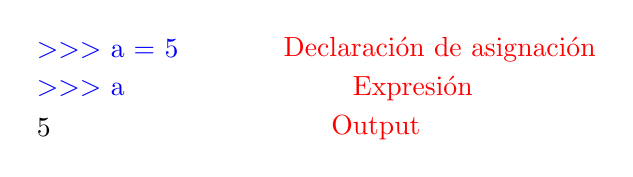
\begin{tikzpicture}[node distance=12em]
\node(A) [anchor=west, text=blue] at (0,1) {$> > >$ a = 5};
\node(B) [anchor=west, text=blue] at (0,0.5) {$> > >$ a};
\node(C) [anchor=west] at (0,0) {5};
\node(A1) [right of=A, text=red]  {Declaraci\'on de asignaci\'on};
\node(A1) [right of=B, text=red]  {Expresi\'on};
\node(C1) [right of=C, text=red]  {Output};
\end{tikzpicture}
\end{minipage}
Note que {\color{blue}a} es una variable tipo \alert{integer} almacenada en la memoria. {\color{blue}a} puede ser utilizada como:
\begin{minipage}[t]{\linewidth}
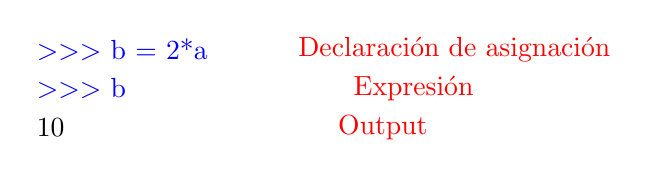
\begin{tikzpicture}[node distance=12em]
\node(A) [anchor=west, text=blue] at (0,1) {$> > >$ b = 2*a};
\node(B) [anchor=west, text=blue] at (0,0.5) {$> > >$ b};
\node(C) [anchor=west] at (0,0) {10};
\node(A1) [right of=A, text=red]  {Declaraci\'on de asignaci\'on};
\node(A1) [right of=B, text=red]  {Expresi\'on};
\node(C1) [right of=C, text=red]  {Output};
\end{tikzpicture}
\end{minipage}
Una variable {\color{blue}a} puede actualizarse:
\begin{minipage}[t]{\linewidth}
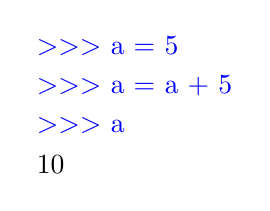
\begin{tikzpicture}
\node [anchor=west, text=blue] at (0,1) {$> > >$ a = 5};
\node [anchor=west, text=blue] at (0,0.5) {$> > >$ a = a + 5};
\node [anchor=west, text=blue] at (0,0) {$> > >$ a};
\node [anchor=west] at (0,-0.5) {10};
\end{tikzpicture}
\end{minipage}
\end{frame}


\begin{frame}[c]{Nombre de las variables}
\begin{itemize}
\item Todas las variables deben comenzar con una letra. Es recomendado iniciar con una letra minuscula.
\item Las siguientes letras pueden ser mayusculas, minusculas o n\'umeros. 
\item Los nombres de las variables son sensibles a las mayusculas y minusculas: 
\begin{minipage}[t]{\linewidth}
\vspace{0,5cm}
\centering
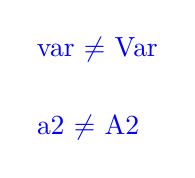
\begin{tikzpicture}
\node(A) [anchor=west, text=blue] at (0,1) {var $\neq$ Var};
\node(B) [anchor=west, text=blue] at (0,0) {a2 $\neq$ A2};
\end{tikzpicture}
\end{minipage}
\end{itemize}
\end{frame}


\begin{frame}[c]{Abreviaciones sintacticas}
\begin{tabular}{c c c}
varname $+=$ 10   & $\equiv$ &  varname $=$ varname $+$ 10 \\
varname $-=$ 10   & $\equiv$ &  varname $=$ varname $-$ 10 \\
varname $*=$ 10   & $\equiv$ &  varname $=$ varname $*$ 10 \\
varname $/=$ 10   & $\equiv$ &  varname $=$ varname $/$ 10 \\
varname $**=$ 10   & $\equiv$ &  varname $=$ varname $**$ 10 \\
varname $\%=$ 10   & $\equiv$ &  varname $=$ varname $\%$ 10
\end{tabular}
\end{frame}

\begin{frame}[c]{Estructuras de datos en Python}
\co{list}: Una lista es una colecci\'on de datos
\begin{itemize}
\item Del mismo o de diferente tipo
\begin{minipage}[t]{\linewidth}
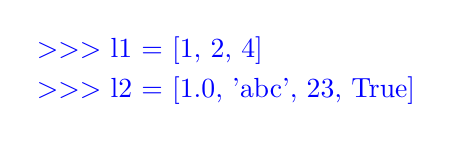
\begin{tikzpicture}
\node [anchor=west, text=blue] at (0,1) {$> > >$ l1 = [1, 2, 4]};
\node [anchor=west, text=blue] at (0,0.5) {$> > >$ l2 = [1.0, 'abc', 23, True]};
\end{tikzpicture}
\end{minipage}
\item Pueden incluir listas dentro de listas
\begin{minipage}[t]{\linewidth}
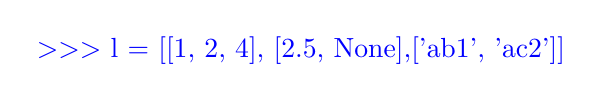
\begin{tikzpicture}
\node [anchor=west, text=blue] at (0,1) {$> > >$ l = [[1, 2, 4], [2.5, None],['ab1', 'ac2']]};
\end{tikzpicture}
\end{minipage}
\item Una lista vacia se expresa como: 
\begin{minipage}[t]{\linewidth}
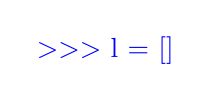
\begin{tikzpicture}
\node [anchor=west, text=blue] at (0,1) {$> > >$ l = []};
\end{tikzpicture}
\end{minipage}
\item Se pueden acceder a los elementos de una lista a trav\'es de indices
\begin{minipage}[t]{\linewidth}
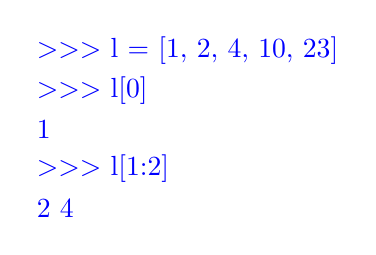
\begin{tikzpicture}
\node [anchor=west, text=blue] at (0,1) {$> > >$ l = [1, 2, 4, 10, 23]};
\node [anchor=west, text=blue] at (0,0.5) {$> > >$ l[0]};
\node [anchor=west, text=blue] at (0,0) {1};
\node [anchor=west, text=blue] at (0,-0.5) {$> > >$ l[1:2]};
\node [anchor=west, text=blue] at (0,-1) {2 4};
\end{tikzpicture}
\end{minipage}
\end{itemize}
\begin{tikzpicture}[overlay]
\node [align=center](A) at (11.3,5.3) {
\begin{tabular}{p{0.1\textwidth} p{0.3\textwidth}}
\co{count()} & Calcula el numero de elementos de una lista.\\
\co{append()} & Adiciona un elemento al final de la lista.\\
\co{clear()} & Remueve todos los elementos de una lista.\\
\co{sort()} & Ordena los elementos de la list.\\
\co{insert()} & Insert elementos en una posici\'on determinada.
\end{tabular}};
\end{tikzpicture}

\end{frame}

\begin{frame}[fragile]{Estructuras de datos en Python}
\begin{minipage}[t]{\linewidth}
\begin{tikzpicture}[overlay]
\node [text width=15cm](A) at (7,2.3) {
\co{dictionary}: Es una colección de elementos, donde cada uno tiene una llave \alert{key} y un valor \alert{value}. Los diccionarios se pueden crear con paréntesis \{\} separando con una coma cada par \co{key: value}. En el siguiente ejemplo tenemos tres keys que son el nombre, la edad y el documento. 
};
\end{tikzpicture}
\end{minipage}
\begin{tikzpicture}[overlay]
\node [align=center](A) at (7,0.2) {
\begin{tabular}{p{0.32\textwidth} p{0.32\textwidth} p{0.32\textwidth}}
\begin{lstlisting}[language=Python]
d1 = {
  "Nombre": "Sara",
  "Edad": 27,
  "Documento": 1003882
}
print(d1)
#{'Nombre': 'Sara', 'Edad': 27, 'Documento': 1003882}
\end{lstlisting}&
\begin{lstlisting}[language=Python]
d2 = dict([
      ('Nombre', 'Sara'),
      ('Edad', 27),
      ('Documento', 1003882),
])
print(d2)
#{'Nombre': 'Sara', 'Edad': '27', 'Documento': '1003882'}
\end{lstlisting}&
\begin{lstlisting}[language=Python, title=Diccionario anidado]
d3 = dict(Nombre='Sara',
          Edad=27,
          Documento=1003882)
print(d3)
#{'Nombre': 'Sara', 'Edad': 27, 'Documento': 1003882}
\end{lstlisting}
\end{tabular}};
\end{tikzpicture}
\end{frame}

\begin{frame}[fragile]{Estructuras de datos en Python}
\begin{tikzpicture}[overlay]
\node [align=center](A) at (7,0.5) {
\begin{tabular}{p{0.32\textwidth} p{0.32\textwidth} p{0.32\textwidth}}
\begin{lstlisting}[language=Python, title=Acceder y modificar elementos]
print(d1['Nombre'])     #Sara
print(d1.get('Nombre')) #Sara

d1['Nombre'] = "Laura"
print(d1)
#{'Nombre': Laura', 'Edad': 27, 'Documento': 1003882}
\end{lstlisting}&
\begin{lstlisting}[language=Python, title=Iterar diccionario]
# Imprime los key y value del diccionario
for x, y in d1.items():
    print(x, y)
#Nombre Laura
#Edad 27
#Documento 1003882
#Direccion Calle 123
\end{lstlisting}&
\begin{lstlisting}[language=Python, title=Diccionario anidado]
anidado1 = {"a": 1, "b": 2}
anidado2 = {"a": 1, "b": 2}
d = {
  "anidado1" : anidado1,
  "anidado2" : anidado2
}
print(d)
#{'anidado1': {'a': 1, 'b': 2}, 'anidado2': {'a': 1, 'b': 2}}
\end{lstlisting}
\end{tabular}};
\end{tikzpicture}
\begin{tikzpicture}[overlay]
\node [align=center](A) at (6,-2.5) {
%M\'etodos y funciones para dictionarios
\begin{columns}
\column{0.99\textwidth}
\begin{itemize}
\item \co{clear()}: Elimina todo el contenido del diccionario.  
\item \co{get(<key>[,<default>])}: Este m\'etodo nos permite consultar el \co{value} para un \co{key} determinado. 
\item \co{items()}: Devuelve una lista con los keys y values del diccionario.
\item \co{keys()}: Devuelve una lista con todas las keys del diccionario.
\item \co{values()}: Devuelve una lista con todos los values del diccionario.
\end{itemize}
\end{columns}};
\end{tikzpicture}
\end{frame}


\begin{frame}[fragile]{Otras estructuras de datos en Python}
\begin{itemize}
\item \co{tuple}: Es una colecci\'on de objetos o variables similar a una \co{list} en donde sus objetos son inmutables. Esto quiere decir que los objetos en un \co{tuple} no puden ser creados o removidos una vez creado el \co{tuple}. E.g. \co{Tuple = ('Geeks', 'For')}.
\item \co{set}: Es una coleccion de datos en python la cual mutable similar a una lista y no permite duplicados de datos. E.g. \co{Set = set([1, 2, 'Geeks', 4, 'For', 6, 'Geeks'])} 
\end{itemize}
\end{frame}
\begin{frame}[fragile]{Condicionales en Python}
\begin{tikzpicture}[overlay]
\node [align=center](A) at (6.5,3) {
\co{if ()} \co{elif:} \co{else:} son usadas para ejecutar expresiones dependiendo de una condicion logica
};
\end{tikzpicture}
\begin{tikzpicture}[overlay]
\node [align=center](A) at (7,0.5) {
\begin{tabular}{p{0.32\textwidth} p{0.32\textwidth} p{0.32\textwidth}}
\begin{lstlisting}[language=Python]
a = 33
b = 200
if b > a:
  print("b is greater than a")
\end{lstlisting}
producira: \co{b is greater than a}&
\begin{lstlisting}[language=Python]
a = 33
b = 33
if b > a:
  print("b is greater than a")
elif a == b:
  print("a and b are equal")
\end{lstlisting}
producira: \co{a and b are equal} &
\begin{lstlisting}[language=Python]
a = 200
b = 33
if b > a:
  print("b is greater than a")
elif a == b:
  print("a and b are equal")
else:
  print("a is greater than b")
\end{lstlisting}
producira: \co{a is greater than b} 
\end{tabular}};
\end{tikzpicture}
\begin{tikzpicture}[overlay]
\node [align=center](A) at (7,-3) {
\begin{tabular}{p{0.49\textwidth} p{0.49\textwidth}}
Formas compactas de escribir condicionales:
\begin{lstlisting}[language=Python]
a = 200
b = 30
if a > b: print("a is greater than b")
\end{lstlisting}
producira: \co{a is greater than b} & 
\begin{lstlisting}[language=Python]
a = 330
b = 330
print("A") if a > b else print("=")
\end{lstlisting}
producira: \co{$=$}
\end{tabular}};
\end{tikzpicture}
\end{frame}

\begin{frame}[fragile]{Condicionales en Python}
\begin{tikzpicture}[overlay]
\node [align=center](A) at (3.8,2.8) {
Uso de operadores logicos \co{and}, \co{or} y \co{not} en condicionales
};
\end{tikzpicture}

\begin{tikzpicture}[overlay]
\node [align=center](A) at (7,1.3) {
\begin{tabular}{p{0.32\textwidth} p{0.32\textwidth} p{0.32\textwidth}}
\begin{lstlisting}[language=Python]
a = 200
b = 33
c = 500
if a > b and c > a:
  print("Both conditions are True")
\end{lstlisting}
producira: \co{Both conditions are True}&
\begin{lstlisting}[language=Python]
a = 200
b = 33
c = 500
if a > b or a > c:
  print("At least one of the conditions is True")
\end{lstlisting}
producira: \co{At least one of the conditions is True} &
\begin{lstlisting}[language=Python]
a = 33
b = 200
if not a > b:
  print("a is NOT greater than b")
\end{lstlisting}
producira: \co{a is NOT greater than b} 
\end{tabular}};
\end{tikzpicture}
\begin{tikzpicture}[overlay]
\node [align=center](A) at (7,-2.5) {
\begin{tabular}{p{0.49\textwidth} p{0.49\textwidth}}
\begin{lstlisting}[language=Python,title=Condicional anidado]
x = 41
if x > 10:
  print("Above ten,")
  if x > 20:
    print("and also above 20!")
  else:
    print("but not above 20.") 
\end{lstlisting}
producira: \co{Above ten,} y \co{and also above 20!}& 
\begin{lstlisting}[language=Python,title=uso de \co{pass}]
a = 33
b = 200
if b > a:
  pass
\end{lstlisting}
\end{tabular}};
\end{tikzpicture}

\end{frame}

\begin{frame}[fragile]{Los \co{for} loops}
\begin{tikzpicture}[overlay]
\node [align=center](A) at (7.3,1.3) {
\begin{tabular}{p{0.32\textwidth} p{0.32\textwidth} p{0.32\textwidth}}
\begin{lstlisting}[language=Python, title=Loop a trav\'es de una \alert{lista}]
fruits = ["apple", "banana", "cherry"]
for x in fruits:
  print(x)
\end{lstlisting}&
\begin{lstlisting}[language=Python, title=Loop a trav\'es de un \alert{string}]
for x in "banana":
  print(x)
\end{lstlisting}&
\begin{lstlisting}[language=Python, title=Uso de \co{break}]
fruits = ["apple", "banana", "cherry"]
for x in fruits:
  print(x)
  if x == "banana":
    break
\end{lstlisting}
\end{tabular}};
\end{tikzpicture}

\begin{tikzpicture}[overlay]
\node [align=center](A) at (7,0) {
\begin{columns}
\column{0.30\textwidth}
producir\'a: \\
\co{apple} \\
\co{banana} \\
\co{cherry}

\column{0.30\textwidth}
producir\'a: \\
\co{b} \\
\co{a} \\
\co{n} \\
\co{a} \\
\co{n} \\
\co{a}

\column{0.30\textwidth}
producir\'a: \\
\co{apple}
\end{columns}};
\end{tikzpicture}

\end{frame}

\begin{frame}[fragile]{Los \co{for} loops}
\begin{tikzpicture}[overlay]
\node [align=center](A) at (7.3,1.3) {
\begin{tabular}{p{0.32\textwidth} p{0.32\textwidth} p{0.32\textwidth}}
\begin{lstlisting}[language=Python, title=Uso de \co{continue}]
fruits = ["apple", "banana", "cherry"]
for x in fruits:
  if x == "banana":
    continue
  print(x) 
\end{lstlisting}&
\begin{lstlisting}[language=Python, title=La funci\'on \co{range()}]
for x in range(6):
  print(x)
\end{lstlisting}&
\begin{lstlisting}[language=Python, title=La funci\'on \co{range()}]
for x in range(2, 30, 3):
  print(x)
\end{lstlisting}
\end{tabular}};
\end{tikzpicture}
\begin{tikzpicture}[overlay]
\node [align=center](A) at (7,-1) {
\begin{columns}
\column{0.30\textwidth}
producir\'a: \\
\co{apple} \\
\co{cherry}

\column{0.30\textwidth}
producir\'a: \\
\co{0} \\
\co{1} \\
\co{.} \\
\co{.} \\
\co{.} \\
\co{5}

\column{0.30\textwidth}
producir\'a: \\
\co{2} \\
\co{5} \\
\co{.} \\
\co{.} \\
\co{.} \\
\co{29}

\end{columns}};
\end{tikzpicture}
\end{frame}

\begin{frame}[fragile]{Los \co{while} loops}
\begin{tikzpicture}[overlay]
\node [align=center](A) at (7.3,1.3) {
\begin{tabular}{p{0.32\textwidth} p{0.32\textwidth} p{0.32\textwidth}}
\begin{lstlisting}[language=Python]
i = 1
while i < 6:
  print(i)
  i += 1
\end{lstlisting}&
\begin{lstlisting}[language=Python, title=Uso de \co{break}]
i = 1
while i < 6:
  print(i)
  if i == 3:
    break
  i += 1 
\end{lstlisting}&
\begin{lstlisting}[language=Python, title=Uso de \co{continue}]
i = 0
while i < 6:
  i += 1
  if i == 3:
    continue
  print(i)
\end{lstlisting}
\end{tabular}};
\end{tikzpicture}
\begin{tikzpicture}[overlay]
\node [align=center](A) at (7,-1) {
\begin{columns}
\column{0.30\textwidth}
producir\'a: \\
\co{1} \\
\co{2}\\
\co{3}\\
\co{4}\\
\co{5}

\column{0.30\textwidth}
producir\'a: \\
\co{1} \\
\co{2} \\
\co{3}

\column{0.30\textwidth}
producir\'a: \\
\co{1} \\
\co{2} \\
\co{4} \\
\co{5} \\
\co{6} 

\end{columns}};
\end{tikzpicture}

\end{frame}

\begin{frame}[c]{Ejercicio}
\begin{block}{Calculo de la profundidad normal ($y_n$) en canales}
Escribir un programa en Python para determinar la profundidad normal ($y_n$) en un canal trapezoidal cuya base ($b$) es 10 $m$, la pendiente longitudinal del canal ($S_o$) es 0.001, la pendiente lateral ($z$) es 2, el factor de rugosidad de Manning ($n$) es 0.013 y el caudal transportado ($Q$) es 30 m$^3$/s, utilizando la \emph{ecuaci\'on de Manning}:
$$
Q = \frac{1}{n}AR^{2/3}S_o^{1/2}
$$
Utilize el m\'etodo de \emph{Newton-Raphson}:
$$
x_{n+1} = x_n - \frac{f(x_n)}{f'(x_n)}
$$
 para resolver la ecuaci\'on de Manning. 
\end{block}
\end{frame}






\begin{frame}[c]{Leer datos externos}
\end{frame}

\begin{frame}[c]{Imprimir datos en Python}
\end{frame}

%---
\section{Graficas en Python}
\begin{frame}[c]{Paquetes}
\end{frame}

\begin{frame}[c]{Graficar datos}
\end{frame}

\begin{frame}[c]{Atributos de las graficas}
\end{frame}

\begin{frame}[c]{Multiples axes en una grafica}
\end{frame}




`



%\begin{frame}[c]{?`Que es \gi?}
%\begin{columns}
%\column{0.6\textwidth}
%\large{
%\begin{block}{\gi}
%\begin{itemize}
%    \item \gi\ es un programa/sistema usado para el control de versiones en proyectos, particularmente, en c\'odigos de computador.
%    \item \gi\ fue inventado en 2005 por Linus Torvalds, creador de \texttt{Linux}, con el fin de manejar proyectos grandes multiusuario (e.g. kernel de \texttt{Linux} escrito en \texttt{C}) de manera eficiente y r\'apida.
%    \item Git est\'a escrito en \texttt{C} y viene por defecto en \texttt{Linux}. Puede ser instalado en \texttt{MS Windows}.
%\end{itemize}
%\end{block}
%}
%\column{0.4\textwidth}
%\begin{center}
% %\begin{figure}
% \includegraphics[width=\textwidth]{linus.jpeg}
% %\vspace{-0.5cm}
% %\caption{\tiny Fuente: https://en.wikipedia.org/wiki}
% %\end{figure}
% \end{center}
%\end{columns}
%\end{frame}	
%%---
%\section{?`Para que sirve \gi?}
%\begin{frame}[c]{?`Para que sirve \gi?}
%%\begin{columns}
%%\column{0.6\textwidth}
%\large{
%\begin{block}{Utilidades de \gi}
%\begin{itemize}
%    \item Trabajo en grandes proyectos con colaboracion de multiples usuarios y servidores.
%    \item Control de cambios lo que permite ir a hacia adelante o hacia atras en la historia del proyecto.
%    \item Sistema distribuido lo que permite que multiples usuarios hagan cambios y sean a la vez servidores del proyecto.
%\end{itemize}
%\end{block}
%}
%\end{frame}	
%
%\begin{frame}[c]{Modelo centralizado Vs \alert{modelo distribuido}}
%\vspace{-0.2cm}
%\begin{center}
% \includegraphics[width=0.87\textwidth]{dist.png}
% \end{center}
%\end{frame}	
%%---
%\section{Tratamiento de cambios en un repositorio en \gi}
%\begin{frame}[c]{Proyecto local en \gi}
%\vspace{-0.2cm}
%\begin{center}
% %\begin{figure}
% \includegraphics[width=0.55\textwidth]{gitp.png}
% %\vspace{-0.5cm}
% %\caption{\tiny Fuente: https://en.wikipedia.org/wiki}
% %\end{figure}
% \end{center}
%%\end{columns}
%\end{frame}	
%
%\begin{frame}[c]{Ciclo de vida de un archivo de un repositorio en \gi}
%%\column{0.4\textwidth}
%\begin{center}
% %\begin{figure}
% \includegraphics[width=0.8\textwidth]{gitf.png}
% %\vspace{-0.5cm}
% %\caption{\tiny Fuente: https://en.wikipedia.org/wiki}
% %\end{figure}
% \end{center}
%%\end{columns}
%\end{frame}	
%
%%---
%\section{\gih}
%\begin{frame}[c]{\gih}
%\begin{columns}
%\column{0.8\textwidth}
%\begin{block}{\gih}
%\begin{itemize}
%    \item \href{http://www.github.com}{\gih} es una p\'agina web de libre acceso para archivar repositorios online.
%    \item Muchos repositorios de codigo abierto como el kernel de Linux usan \gih.
%    \item ?`Es necesario tener \gih\ para usar \gi? \textbf{No!}
%    \begin{itemize}
%        \item Se puede usar \gi\ localmente, o  
%        \item se puede configurar un servidor para compartir archivos.
%    \end{itemize}     
%\end{itemize}
%\end{block}
%\column{0.2\textwidth}
%\begin{center}
% \includegraphics[width=0.8\textwidth]{ghub.png}
% \end{center}
%\end{columns}
%\end{frame}
%
%
%%---
%\section{Commandos b\'asicos en \gi}
%\begin{frame}[c]{Workflow b\'asico en \gi}
%\begin{block}{Workflow b\'asico en \gi}
%\begin{enumerate}
%    \item \alert{Pull} el directorio \gi\ del servidor remoto (opcional).
%    \item \alert{Modificar} los archivos en el directorio de trabajo
%    \item \alert{Stage} archivos. Adicionar un copia del archivo a la staging area.
%    \item Hacer un \alert{commit}, el cual toma los archivos en la staging area y archiva la copia en el directorio de \gi. 
%    \item \alert{Push} el directorio \gi\ a el servidor remoto (opcional).
%\end{enumerate}
%\end{block}
%\begin{center}
% \includegraphics[width=\textwidth]{workflow.png}
%\end{center}
%\end{frame}	
%
%\begin{frame}[c]{Configuraci\'on inicial en \gi}
%\begin{block}{Alistarse para usar \gi}
%    \begin{enumerate}
%    \item Introducir \texttt{username} y \texttt{email} para ser usado por \gi\ cuando se haga un \texttt{commit}.\\
%     \co{\$ git config --global user.name “Luis Morales”}\\ %\vspace{0.3cm}
%     \co{\$ git config --global user.email lmoralesm@unal.edu.co}
%     \begin{itemize}
%         \item Para verificar la configuraci\'on:\\
%              \co{\$ git config -list}
%         \item Esta configuraci\'on es para todos los proyectos \gi.
%         \item La configuraci\'on anterior puede ser para un proyecto determinado si no se usa la opci\'on \co{-{}-global}
%         \item Adem\'as en la configuraci\'on inicial se puede escoger el editor para escribir mensajes en commit:
%         \co{\$ git config -{}-global core.editor vim}
%     \end{itemize}
%    \end{enumerate}
%\end{block}
%\end{frame}	
%
%\begin{frame}[c]{Crear una copia local del repositorio}
%\begin{block}{Crear copia local del repositorio \gi}
%\begin{enumerate}
%    \item Dos escenarios posibles:
%    \begin{enumerate}
%        \item Clonar un repositorio existente en su directorio local:\\
%        \co{\$ git clone <url> [local\_dir\_name]}\\
%        Crea el directorio \texttt{local\_dir\_name}, el cual contiene una copia de los archivos del repo original, y un directorio \texttt{.git}.
%        \item Crear un repositorio \gi\ en el directorio actual:\\
%        \co{\$ git init}\\
%        Crea el directorio \texttt{.git} en el directorio actual.  
%    \end{enumerate}
%\end{enumerate}
%\end{block}
%\end{frame}	
%
%\begin{frame}[c]{Commit archivos}
%\begin{block}{Commit archivos en el repo local}
%\begin{enumerate}
%    \item Una ves creado el directorio, se puede:
%    \begin{enumerate}
%        \item Se pueden crear archivos dentro del repositorio y adicionarlos a la staging \'area: \\
%        \co{\$ git add README.md file1.c}\\
%        Toma un snapshop de estos archivos en este instante de tiempo y los adiciona a la staging \'area.
%        \item Commit cambios en el repo (mover los staged cambios al repo)
%        \co{\$ git commit -m "initial project version"}\\
%    \end{enumerate}
%    Para unstage cambios (deshacer cambios) en un archivo antes de commit este):\\
%    \co{\$ git reset HEAD -{}- filename}
%    Para deshacer cambios en un archivo despu\'es de commit este:\\
%    \co{\$ git checkout -{}- filename}
%\end{enumerate}
%\end{block}
%\end{frame}	
%
%\begin{frame}[c]{Status y Diff}
%\begin{block}{Status y Diff}
%\begin{itemize}
%    \item Para mirar el \texttt{status} de los archivos en el directorio de trabajo o repo y la staging area:\\
%    \co{\$ git status} o \\
%    \co{\$ git status -s}\\
%    donde la opci\'on \co{-s} muestra una versi\'on del archivo en la staging \'area.
%    \item Para ver cual archivo ha sido modificado pero no est\'a en la staging \'area:\\
%    \co{\$ git diff}
%    \item Para ver cambios que ya estan en la staging \'area:\\
%    \co{\$ git diff}
%\end{itemize}
%\end{block}
%\end{frame}	
%
%\begin{frame}[c]{Chequeando los \texttt{logs}}
%\begin{block}{Chequeando los \texttt{logs}}
%\texttt{log} es un comando en \gi\ que permite conocer los cambios hechos en el repo. Algunos comandos importantes:
%\begin{itemize}
%    \item Chequeando la versi\'on larga de \texttt{logs}:\\
%    \co{\$ git log}
%    \item Chequeando la versi\'on larga de \texttt{logs}:\\
%    \co{\$ git log -{}-oneline}
%    %\begin{center}
%    %\includegraphics[width=\textwidth]{}
%    %\end{center}
%    \item Para mostrar los 5 m\'as recientes cambios:\\
%    \co{\$ git log -5}
%\end{itemize}
%Notas:
%\begin{enumerate}
%    \item Los cambios son listado de acuerdo con el commitID \#.
%    \item Todos los cambios hechos en el repo antes de haber sido clonado o jalado estan incluidos en \texttt{logs}.  
%\end{enumerate}
%\end{block}
%\end{frame}	
%
%\begin{frame}[c]{Pulling y pushing}
%\begin{block}{Pulling y pushing}
%\texttt{pull} y \texttt{push} son dos comandos que permiten jalar el repo de un servidor externo y enviar cambios a el repo, respectivamente. Buenas pr\'acticas en el uso de estos comandos son:
%\begin{enumerate}
%    \item \texttt{Add} y \texttt{commit} los cambios al repo local.
%    \item \texttt{pull} del repo remoto para obtener los cambios mas recientes. En caso de conflictos, \texttt{add} y \texttt{commit} estos al repo. 
%    \item \texttt{push} los cambios al repo remoto.
%\end{enumerate}
%Para incluir los cambios m\'as recientes del repo remoto en el repo local:\\
%\begin{enumerate}
%    \item Para bajar el contenido del repo remoto al repo local (optional):\\
%    \co{\$ git fetch}
%    \item Para bajar el contenido del repo remoto y actualizar el repo local:\\
%    \co{\$ git pull origin master}\\
%\end{enumerate}
%Para \texttt{push} los cambios realizados en el repo local a el repo remoto:\\
%\co{\$ git push origin master}
%\end{block}
%\end{frame}	
%
%\begin{frame}[c]{Branching}
%\vspace{-0.3cm}
%\begin{block}{Branching}
%\texttt{branch} es un comando que permite crear ramificaciones dentro del repo local para hacer cambios experimentales en el.
%\begin{itemize}
%    \item Para crear un \texttt{branch} llamado e.g. experiment1:\\
%    \co{\$ git branch experiment1}
%    \item Para listar todos los branches en el repo:\\
%    \co{\$ git branch}\\
%    Note que * indica el branch actual
%    \item Para cambiar al branch \texttt{experiment1}:\\
%    \co{\$ git checkout experiment1}
%    \item Para introducir los cambios hechos en  \texttt{experiment1} dentro del branch \texttt{master}:\\
%    \co{\$ git checkout master}\\
%    \co{\$ git merge experiment1}      
%\end{itemize}
%Notas:
%\begin{enumerate}
%    \item \co{\$ git log -{}-graph} puede ser usado para mostrar los branches gr\'aficamente. 
%    \item Los branches est\'an solo en el repo local.
%\end{enumerate}
%\end{block}
%\end{frame}	
%
%\begin{frame}[c]{Resumen}
%\vspace{-0.2cm}
%\begin{block}{Resumen}
%Configuraci\'on inicial y clonaci\'on
%\begin{enumerate}
%    \item \co{\$ git config -{}-global user.name “Your Name”}
%    \item \co{\$ git config --global user.email youremail@unal.edu.co}
%    \item \co{\$ git clone https://github.com/hydsrg/hyds-repo.git}
%\end{enumerate}
%Editar y visualizar cambios \texttt{hyds-repo}
%\begin{enumerate}
%    \item \co{\$ git log}; \co{\$ git log -{}-oneline}
%    \item Create a file, e.g. \texttt{filename.txt}
%    \item \co{\$ git status}; \co{\$ git status –s}
%    \item Agregar el archivo al repo (staging area): \co{git add filename.txt}
%    \item \co{\$ git status}; \co{\$ git status –s}
%    \item \texttt{commit} el archivo al repo local:\\
%    \co{\$ git commit –m “added filename.txt file”}
%    \item \co{\$ git status}; \co{\$ git status –s}; \co{\$ git log -{}-oneline}
%\end{enumerate}
%\end{block}
%\end{frame}	
%
%\begin{frame}[c]{Resumen}
%\begin{block}{Resumen}
%Pulling y pushing los cambios
%\begin{enumerate}
%    \item \texttt{pull} de un repo remoto: \co{\$ git pull origin master}
%    \item \texttt{push} hacia un repo remoto: \co{\$ git push origin master}
%\end{enumerate}
%\end{block}
%\end{frame}	

\end{document}



